\documentclass[10pt,twocolumn]{article}
\usepackage{times}
\usepackage{graphicx}
\usepackage{amssymb}
\usepackage{titling}
\usepackage{url,hyperref}

\begin{document}

\title{Spectral Clustering}

\author{Dror Ayalon (dda290)}

\date{%
CUSP-GX-5006 Machine Learning for Cities (NYU)\\
Assigment \# 4\\
\rule{\textwidth}{1pt}
}

\posttitle{\par\rule{3in}{0.4pt}\end{center}\vskip 0.5em}
% \postdate{\rule{\textwidth}{1pt}}

\maketitle

\begin{abstract}
  This report show a comparison between three clustering techniques: Spectral Clustering, K-means, and Hierarchical Clustering. Given the dataset that was used for this report, the most accurate techniques were found to be Spectral Clustering (when using 'lobpcg' as the eigen solver, and considering 25 neighbors when constructing the affinity matrix), and Hierarchical Clustering (when computing the linkage using the 'cosine' method, and using an 'average' as  a linkage cretirion).
\end{abstract}

\section{Methods and Data Sets}
\begin{enumerate}

  \begin{figure}[!t]
    \begin{center}
      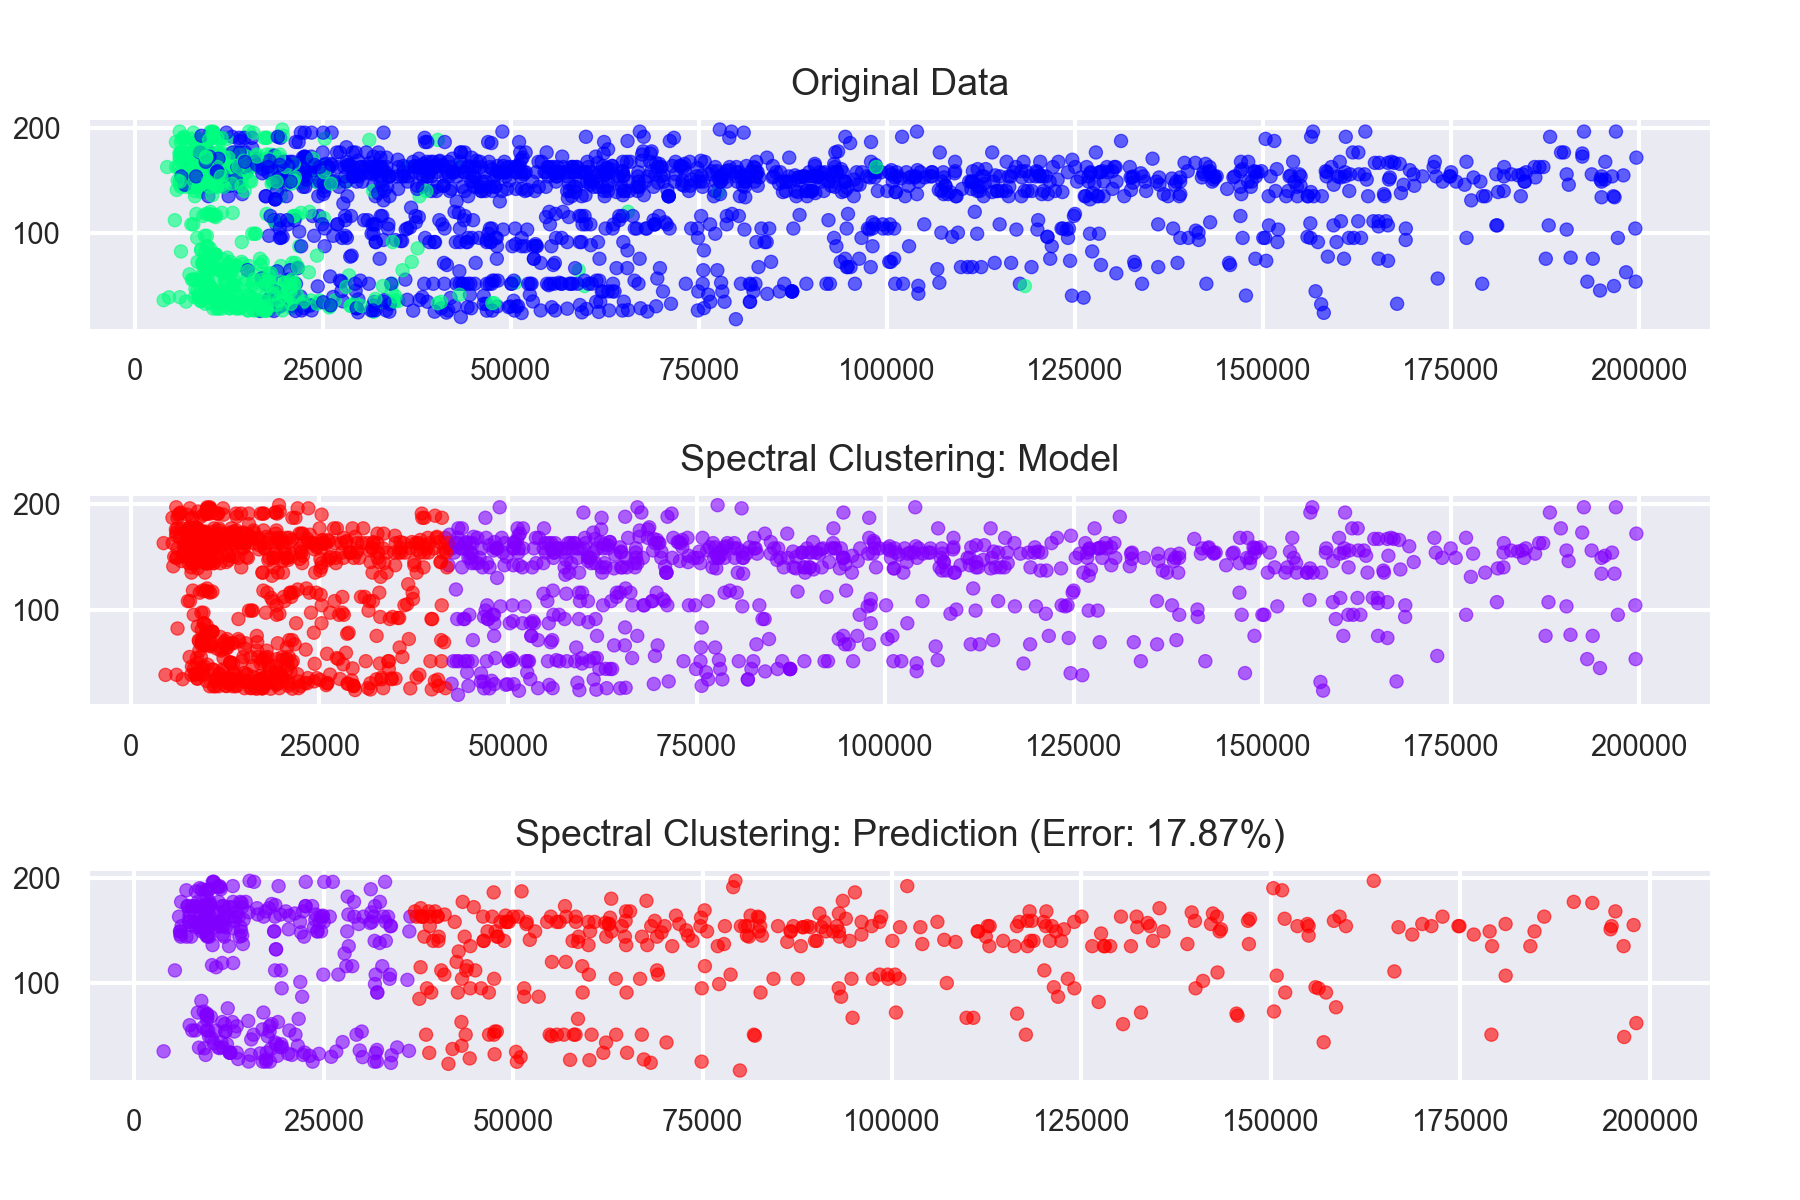
\includegraphics[width=3in]{../plots/spectral.png}
    \end{center}
    \label{spectral}
    \caption{\small Raw data VS. model genrated by a Spectral Clustering algorithm VS. the most accurate prediction by the Spectral Clustering algorithm}
  \end{figure}

  \item The dataset used for this study is 'manhattan-dof.csv', which was made available to us by NYU. The dataset includes 2645 samples. The attributes that were used from this dataset are the following:
  \begin{itemize}
    \item BldClassif - Building class. Used as a cluster indicator for validation purposes.
    \item GrossSqFt, MarketValueperSqFt - Indipendent variables that were used to generate the prediction model.
    \item I seems that the data that was very hard to cluster, and in most cases, the model that was generated by the algoritms, which are being described below, was not accurate in describing the raw data.
  \end{itemize}

  \item The data was cleaned to remove outlies.

  \item The entire study was done using Python3 and the machine learning Python package scikit-learn (http://scikit-learn.org/).

  \item To validate the results, a cross-validation process was used, based on the 'train\_test\_split' method of the scikit-learn package. During the process, 5 batches of data were generated. 4 of which were used as training sets and 1 was used as a validation set. The random split process was done 50 times for each classfication method. Moreover, a Bootstraping procedure was used to improve the restuls of a few of the classification algorithms. This topic will be discussed below.



  \item The following scikit-learn algorithms were used to the generate the results for this study:
  \begin{figure}[!t]
    \begin{center}
      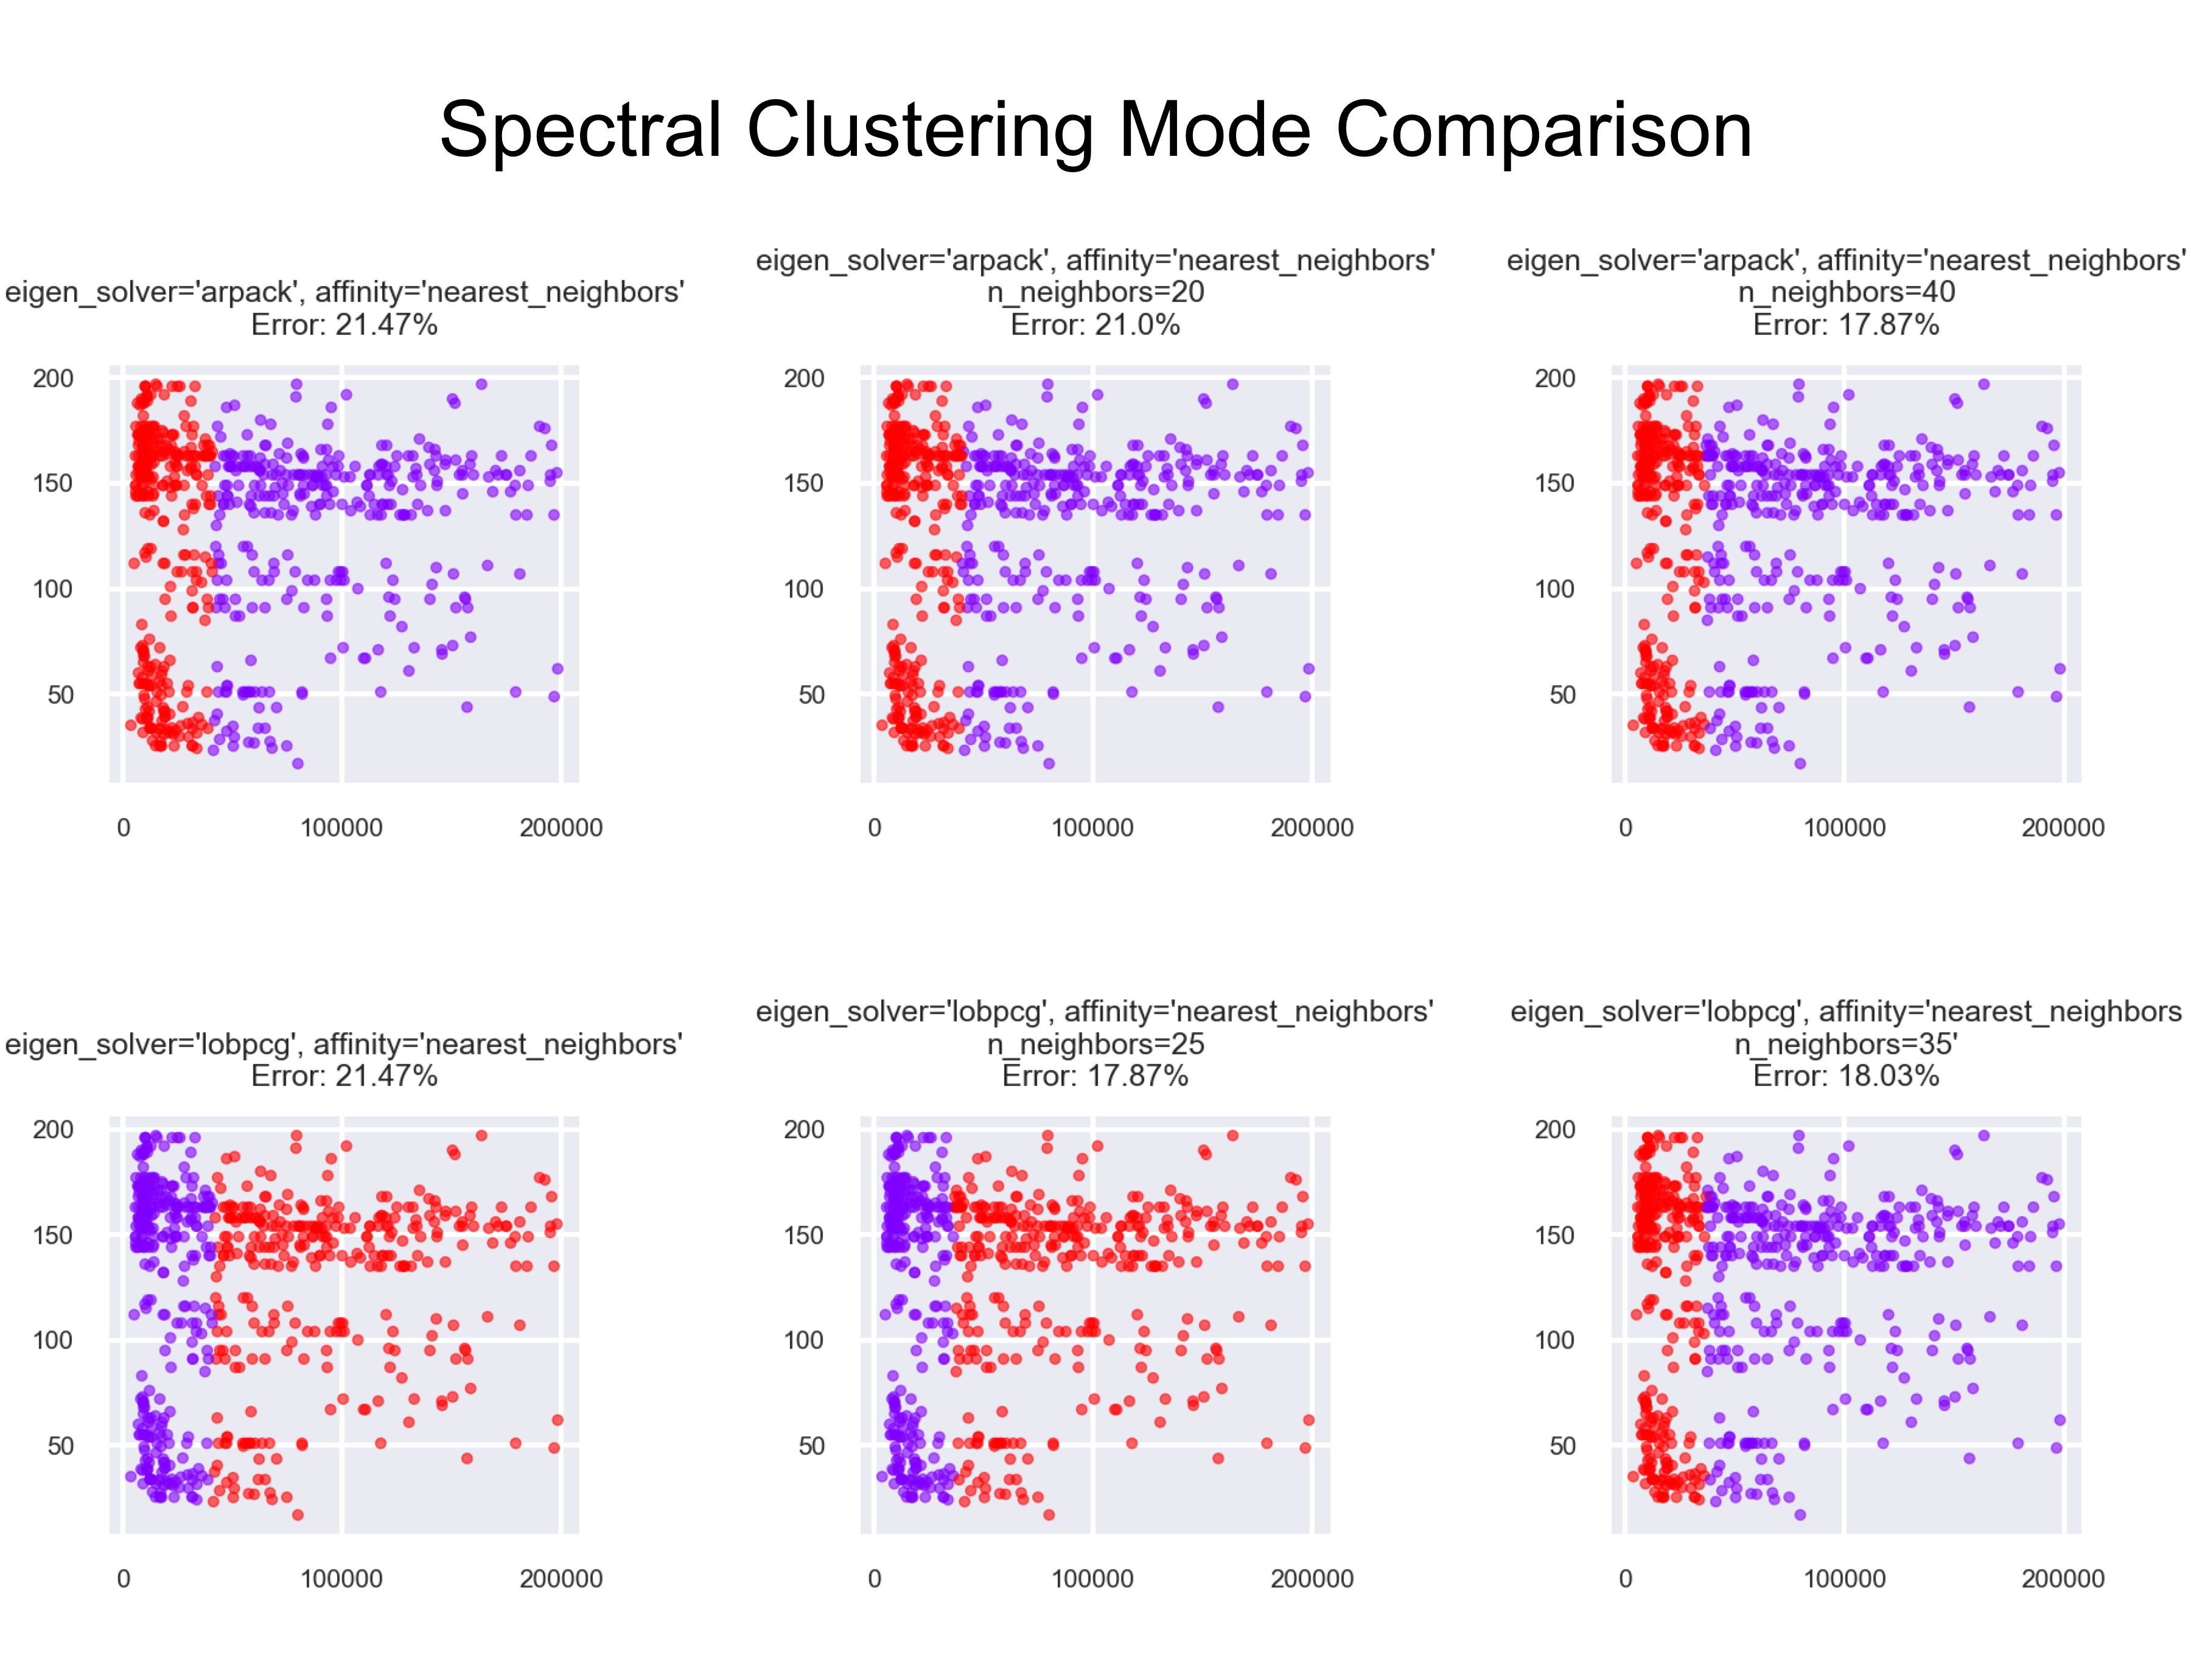
\includegraphics[width=3in]{../plots/spectral_all.png}
    \end{center}
    \label{spectral_all}
    \caption{\small A comparison between different configurations of the Spectral Clusteing algorithm.}
  \end{figure}
    \begin{itemize}
      \item sklearn.cluster.SpectralClustering - Was used to cluster the data using a Spectral Clustering algorithm. This algorithm, using when using 'lobpcg' as the eigen solver and considering 25 neighbors when constructing the affinity matrix, was found to be effective an relatively accurate (comparing to other results) in modeling the clusters in the raw data, and therefore, the prediction model was relatively accurate (see figure~\ref{spectral}).

          \begin{figure}[!t]
            \begin{center}
               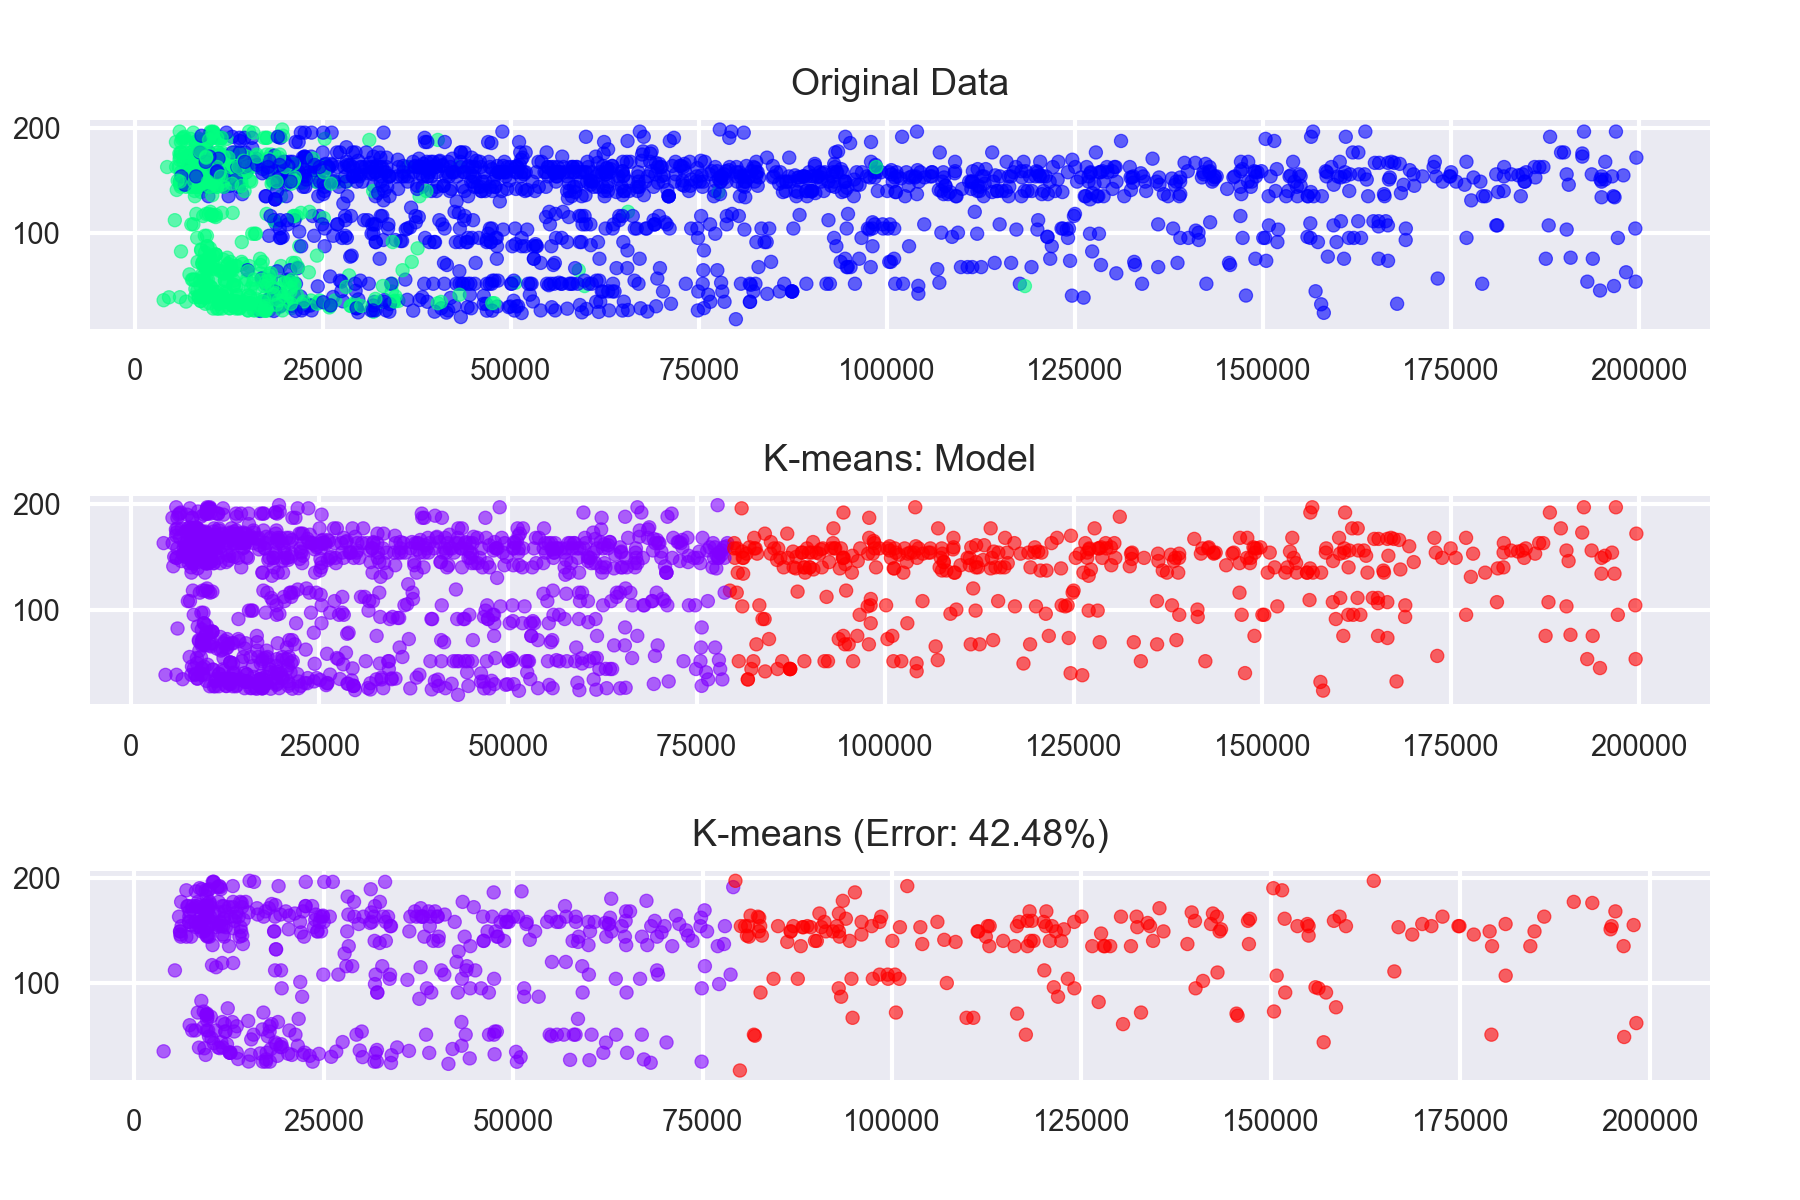
\includegraphics[width=3in]{../plots/k-means.png}
            \end{center}
            \label{k-means}
            \caption{\small Raw data VS. model genrated by a K-means Clustering algorithm VS. the most accurate prediction by the K-means Clustering algorithm}
          \end{figure}


      \item sklearn.cluster.KMeans - Was used to cluster the data using a K-means algorithm. This algorithm was performing poorly in generating an accurate model of the raw data (probably because of the randomality of the data). Therefore, even-though the prediction is relatively accurate comparing to the model, it is still far away from the raw data (see figure~\ref{k-means}).

      \item sklearn.cluster.AgglomerativeClustering - Was used to cluster the data using an Hierarchical algorithm. Even-though this algorithm, when computing the linkage using the 'cosine' method and using the 'average' as a linkage cretirion, showed identical results to those of the Spectral Clustering algorithm, it generated a model that is quite different from the one that was generated by the Spectral Algorithm (see figure~\ref{hierarchical}).

    \end{itemize}

\end{enumerate}



\section{Results}
\begin{itemize}
  \item The result of running a comparison between all the tested algorithms shows a similarity in accuracy between the Spectral Clustering algorithm and the Hierarchical Clustering algorithm (tied at 17.87\% miss clustered samples, see figure~\ref{results}).
  \item Since the data that was used was not very easy to cluster, it is easy to assume that different dataset could yield different results.
\end{itemize}

\begin{figure*}[!b]
  \begin{center}
    \includegraphics[width=3in]{../plots/hierarchical.png}
  \end{center}
  \label{hierarchical}
  \caption{\small Raw data VS. model genrated by a Hierarchical Clustering algorithm VS. the most accurate prediction by the K-means Clustering algorithm}
\end{figure*}

\begin{figure*}[!b]
  \begin{center}
    \includegraphics[width=3in]{../plots/hierarchical_all.png}
  \end{center}
  \label{hierarchical_all}
  \caption{\small A comparison between different configurations of the Hierarchical Clusteing algorithm.}
\end{figure*}

\begin{figure*}[!b]
  \begin{center}
    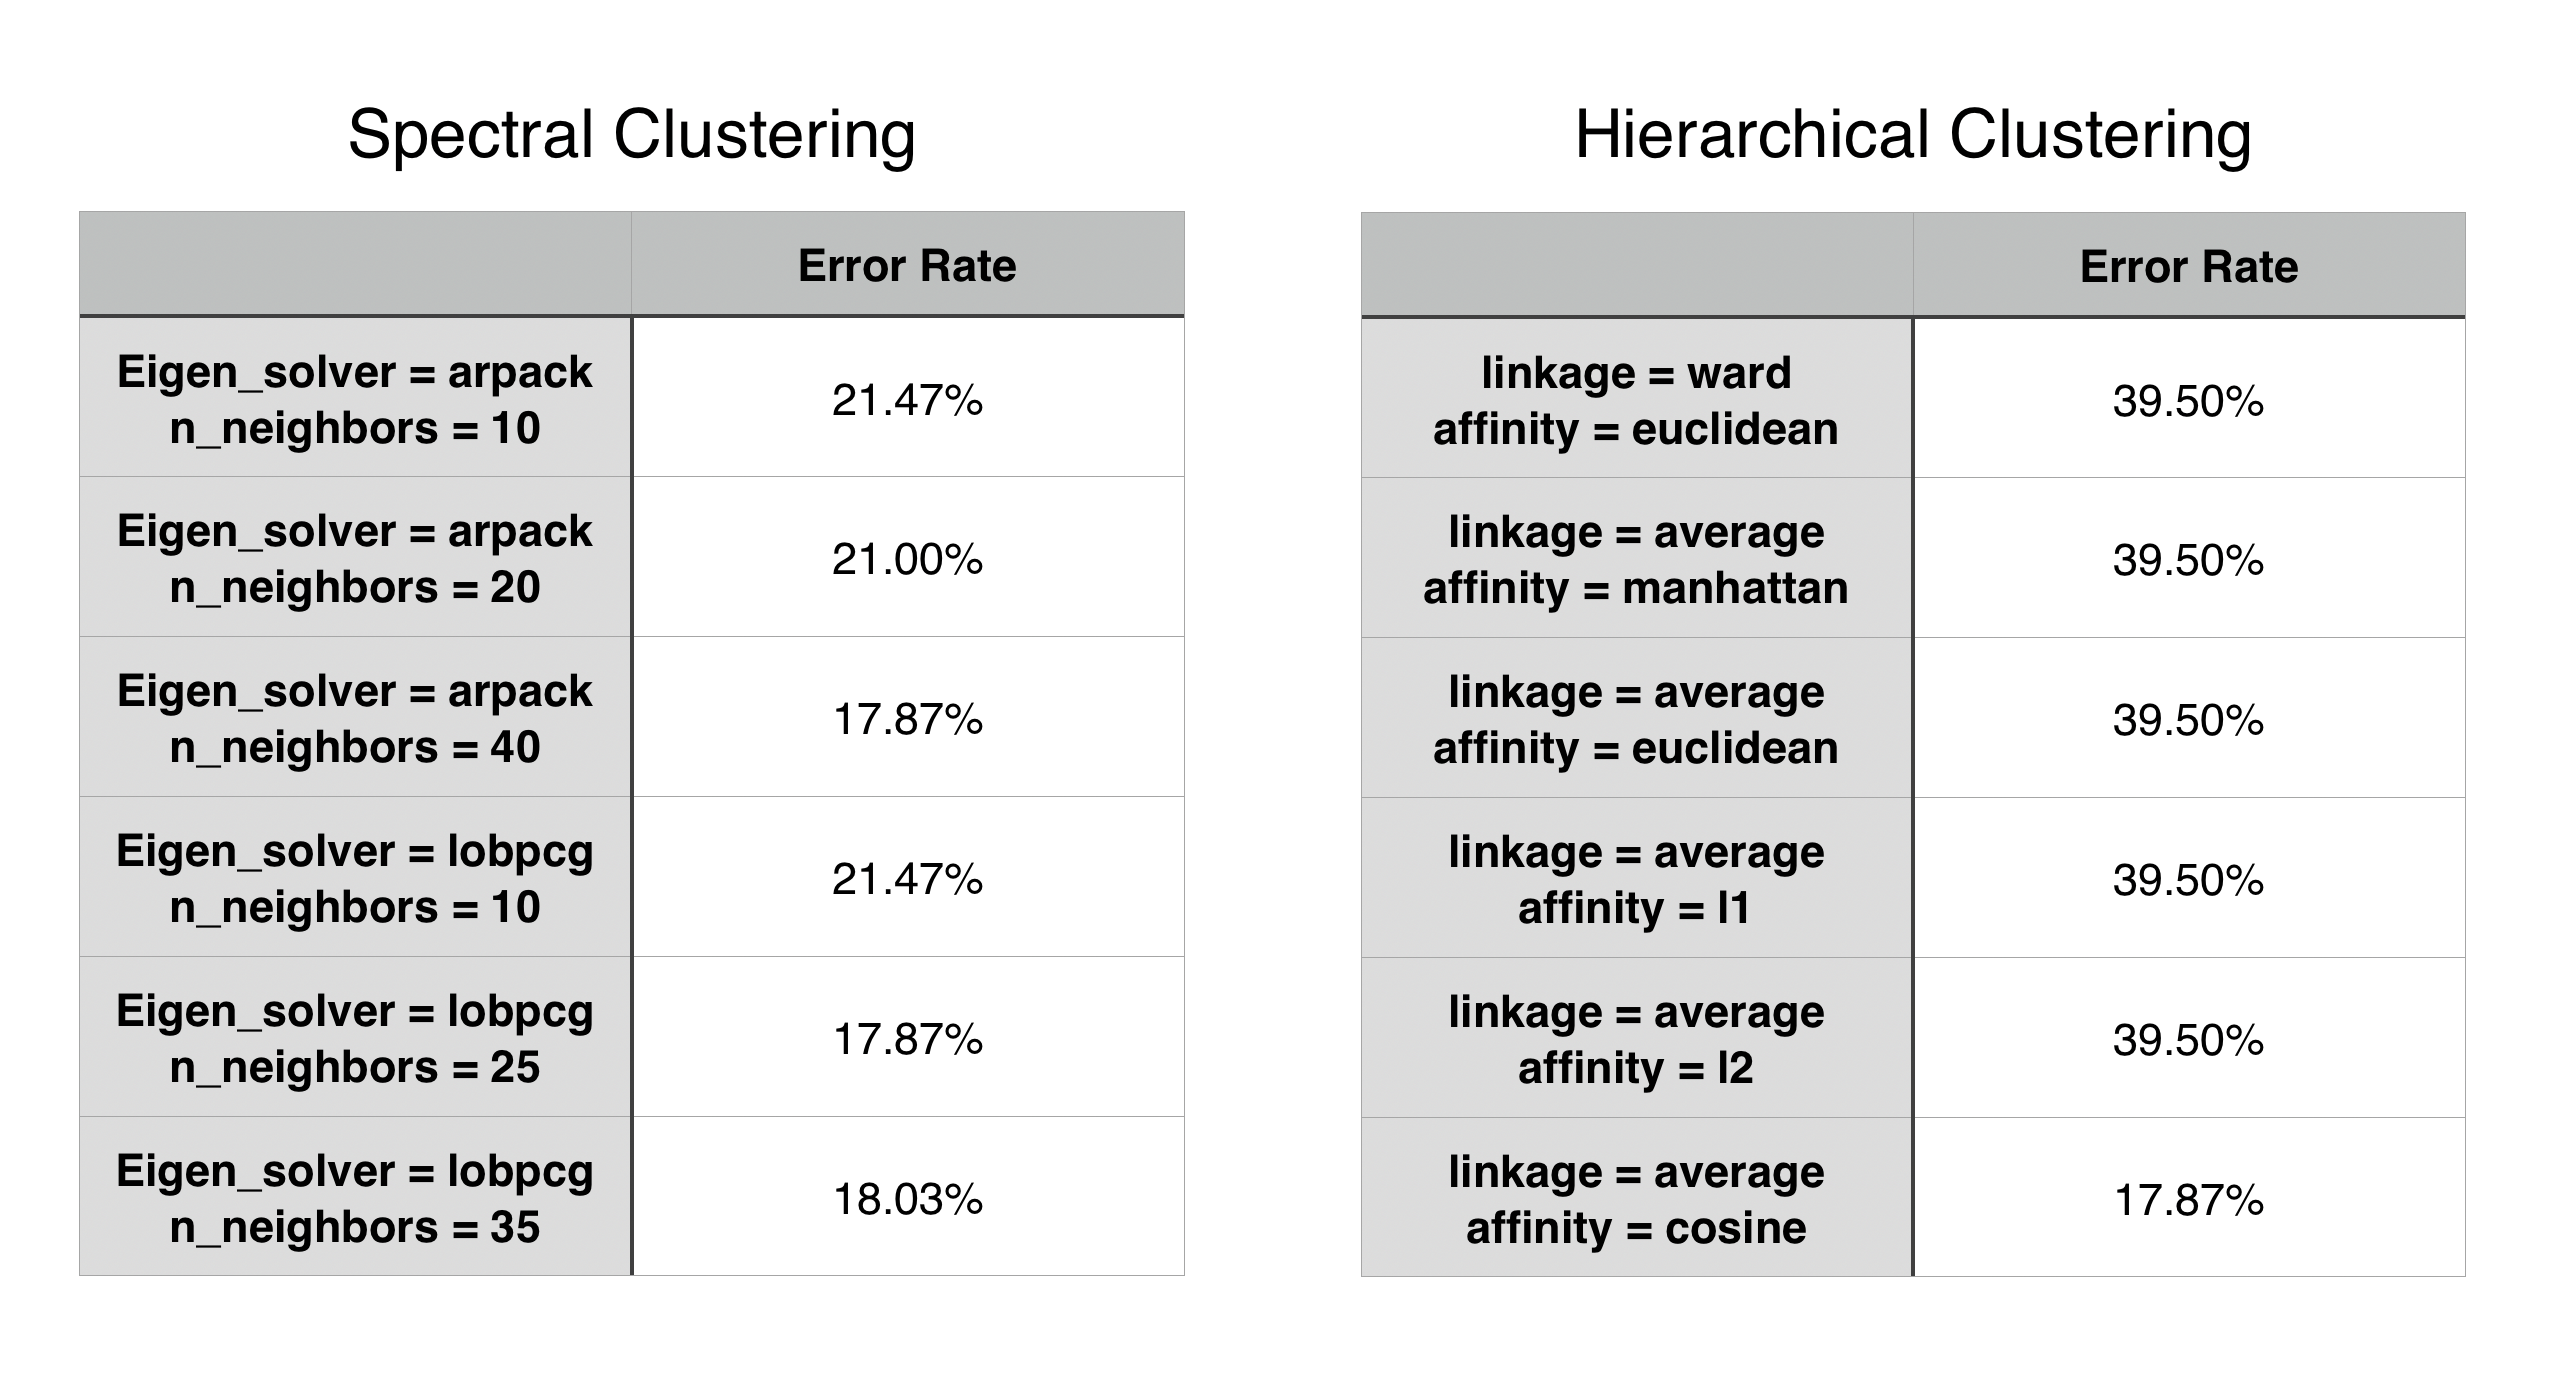
\includegraphics[width=6in]{../plots/results.png}
  \end{center}
  \caption{\small A comparison between error rates of different clustering methods.}
  \label{results}
\end{figure*}


\end{document}
